\documentclass[../../main.tex]{subfiles}

\begin{document}

Every robot needs a drivetrain.

\section{H-Drive}

A H-Drive consists of 4 Omni-Wheels Parallel to each other layed out in the
format of a tank drive. Then in the middle there is a aditional Omni-Wheel
perpendicular to the others.\par

Because of this an H-Drive is holonomic (can move in any direction) because when
the robot goes forward, the 4 main wheels are powered and the rollers on the secondary
wheel can slide to allow the robot to roll forward. \par

Similarly to move sidewast the secondary wheel gets powered. At the same time the rollers on
the main wheels roll to allow the robot to move. By combining the forward movement and sideways
movement, the H-Drive can move in any direction.

\begin{figure}[h]
	\centering
	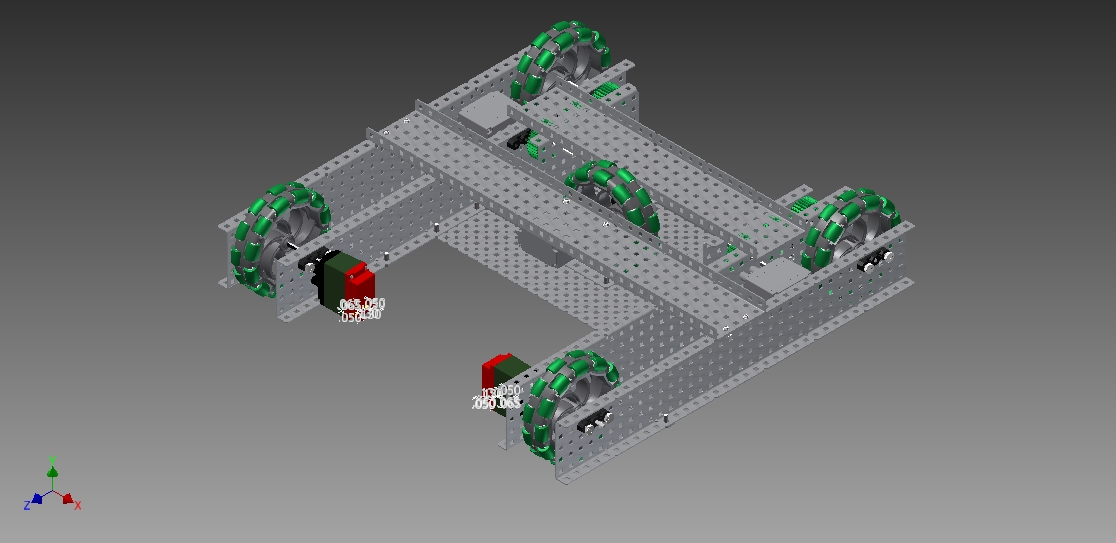
\includegraphics[width=\textwidth]{drivetrains/h}
	\caption{A Typical H-Drive}
	\label{fig:drivetrainh}
\end{figure}

\subsection{Advantages}

\begin{itemize}
	\item Holonomic (can move any direction)
\end{itemize}


\subsection{Disadvantages}

\begin{itemize}
	\item Easy to push sideways as only one wheel is providing
	      traction in that direction.
\end{itemize}


\section{<++>}

<+descirption of drivetrain+>

\begin{figure}
	\centering
	\includegraphics{drivetrains/<+file+>}
	\caption{<+caption text+>}
	\label{fig:drivetrain<+label+>}
\end{figure}

\subsection{Advantages}

\begin{itemize}
	<++>
\end{itemize}


\subsection{Disadvantages}

\begin{itemize}
	<++>
\end{itemize}



\section{<++>}

<+descirption of drivetrain+>

\begin{figure}
	\centering
	\includegraphics{drivetrains/<+file+>}
	\caption{<+caption text+>}
	\label{fig:drivetrain<+label+>}
\end{figure}

\subsection{Advantages}

\begin{itemize}
	<++>
\end{itemize}


\subsection{Disadvantages}

\begin{itemize}
	<++>
\end{itemize}


\section{<++>}

<+descirption of drivetrain+>

\begin{figure}
	\centering
	\includegraphics{drivetrains/<+file+>}
	\caption{<+caption text+>}
	\label{fig:drivetrain<+label+>}
\end{figure}

\subsection{Advantages}

\begin{itemize}
	<++>
\end{itemize}


\subsection{Disadvantages}

\begin{itemize}
	<++>
\end{itemize}





\section{<++>}

<+descirption of drivetrain+>

\begin{figure}
	\centering
	\includegraphics{drivetrains/<+file+>}
	\caption{<+caption text+>}
	\label{fig:drivetrain<+label+>}
\end{figure}

\subsection{Advantages}

\begin{itemize}
	<++>
\end{itemize}


\subsection{Disadvantages}

\begin{itemize}
	<++>
\end{itemize}



\section{<++>}

<+descirption of drivetrain+>

\begin{figure}
	\centering
	\includegraphics{drivetrains/<+file+>}
	\caption{<+caption text+>}
	\label{fig:drivetrain<+label+>}
\end{figure}

\subsection{Advantages}

\begin{itemize}
	<++>
\end{itemize}


\subsection{Disadvantages}

\begin{itemize}
	<++>
\end{itemize}



\end{document}
